\documentclass[12pt]{article}
\usepackage{latexsym}
\usepackage{amssymb,amsmath}
\usepackage[pdftex]{graphicx}


\topmargin = 0.1in \textwidth=5.7in \textheight=8.6in

\oddsidemargin = 0.2in \evensidemargin = 0.2in


\begin{document}

\begin{center}
Applied Mathematics 115, FALL 2015 \\


Theresa Bischoff, Steven Petterutti, Tina Qian, Varun Sriram

\medskip

\textbf{ODE Modeling Age of Empires}


\end{center}

\begin{abstract}
	We modeled the game "Age of Empires," in which rival civilizations attempt to achieve world domination by destroying one another. Our goal is to consider different game strategies and to optimize conditions against enemy AI. By modeling the interaction between two civilizations with sets of ODEs for various strategies, and by performing stability/parameter analysis, we determined the necessary conditions for staying alive and ultimately, winning the game. We found that $\cdots$ TODO
	
\end{abstract}

\section{Introduction}
\paragraph{}
In "Age of Empires," civilizations are pitted against one another, with the objective of winning the game by having the enemy surrender. Each cilization is limited to a certain population size by the game, a "carrying capacity" of typically $200$. Population is split between villagers and military, a designation decided at birth. Villagers gather resources that can be used for births - essentially, villagers can be thought of as the only ones "reproducing." In the game, reproducing can in theory happen infinitely, since structures such as Mills provide a source of infinite resources. Military units are harder to kill and are also the only ones that can attack and kill enemy units. Finally, note that natural births do not exist in the game - if no one is killed, no one dies. \par
In our analysis, we let civilization $C_1$ represent our civilization and civilization $C_2$ represent the enemy AI civilization. We let $C_1 = M_1 + V_1$ and $C_2 = M_2 + V_2$ where the $M_i$ and $V_i$ represent military and villager populations respectively for civilization $i$. The AI civilization surrenders when their numbers fall below a certain threshold $T$, or when our population stabilizes at some nonzero value (the enemy will never be able to kill all our units) - these are conditions for the AI to surrender embedded in the code for the game. \par
When initializing a game, setting certain parameters to specific values can maximize our chances of defeating the AI civilization - these include initial populations of the AI, AI intelligence level and military skills, new unit spawn speed, and map size. Furthermore, parameters such as how fast we click to destroy military units (that is parameter dictating our game performance) can also maximize or hurt our chances defeating the AI civilization. In this project, by exploring models of game strategy, considering phase diagrams, and exploring initial conditions/ parameter sensitivity, we gain insight into what we should set these parameters to, and thus what we can do to maximize our chances of winning. \par

\section{The Model}
\paragraph{}
We consider 3 separate scenarios of increasing complexity. 

\subsection{Scenario 1}

In our first scenario, $C_2$, the enemy AI civilization, starts off with only military. We, $C_1$, choose the strategy of only producing villagers, and not budgeting any reproductive resources to the military. This leads to a model similar to predator prey. \par

$M_1(0) = 0$, $V_1(0)$ and $M_2(0)$ are initial conditions we can vary when initializing the game, and $V_2(0) = 0$.

$$\dot V_1=\alpha V_1(1-\frac{V_1}{k})-V_1(\frac{M_2^2}{A^2+M_2^2})$$
$$ \dot M_i = 0 \text{ for } i \in \{1, 2\} $$
$$\dot V_2 = 0$$

Let us explain our reasoning for the equation for $\dot V_1$. The first term represents logistic growth, such that the carrying capacity is set at $k=200$ by the game code, and the reproduction rate $\alpha$ is determined by (1) what we set the military/villager spawn rate to when initializing the game and (2) how quickly we can click on villagers to gather resources, since the sooner we get more resources, the faster we can create a new villager. The second term represents the predation term where $V_1$ represents the limit that $M_2$ can kill (also ensures that $\dot V_1$ falls to 0 when $V_1 = 0$) and $A$ represents the point at which predation rapidly increases as it is easier to find and kill with more units. Note that $A$ will need to be larger with larger map sizes, and by setting the map size parameter when initializing a game, we effectively vary $A$. In this scenario, we have 2 parameters and 2 initial conditions that we may vary, and $\dot C_1 = \dot V_1$ while $\dot C_2 = 0$. We will investigate what initial conditions and parameter combinations will lead to our victory. In this case, we can win only by stabilizing at a nonzero population in the long run, since we have no military.


\subsection{Scenario 2}

In our second scenario, we initialize the game again so that the AI civilization $C_2$ starts off with only military. However, we, $C_1$, choose now to produce both military and villagers. It is now possible for us to win by either stabilizing our long-run population to be nonzero or wiping out the AI population to $T$. Without loss of generality, let $T = 0$. \par


$$\dot M_1=a \alpha V_1(1-\frac{V_1}{K-V_1})-[M_1D_1(\frac{M_2^2}{A+M_2^2})(\frac{M_1}{A+M_1^3})]$$
$$\dot V_1=(1 - a) \alpha V_1(1-\frac{V_1}{K-M_1})-[V_1cD_1(\frac{M_2^2}{A+M_2^2})(\frac{M_1}{A +M_1^2})]$$
$$\dot M_2=-M_2 D_2(\frac{M_1^2}{A+M_1^2})(\frac{M_2}{A +M_2^3}) $$
$$\dot V_2 = 0 $$

Here, we have that $a$ and $\alpha - a$ to represent the idea that the total reproduction rate $\alpha$ is split into villager births $a$ and military births $\alpha - a$. We maintain logistic growth dependent on $V_1$ but add the $K - X$ term in the denominators to model that carrying capacity for $C_1$ is $K$. We derived the predation terms by holding $\cdots$ TODO NOTE $c = 6$ because it's easier to kill villagers, specifically in the game miltary units have 6x life points. 6 PARAMS total

\subsection{Scenario 3}

 In our final scenario, civilization 2 is permitted to start with some villagers and devotes a portion of new citizens to become villagers. Civilization does not change from the previous case, having both military and villagers. In our final case, we have $C_1 = M_1 + V_1$, with $M_1(0)$ and $V_1(0)$ representing the starting military and villager populations respectively for the first civilzation. However, $C_2 = M_2 + V_2$ as well now, with $M_2(0)$ and $V_2(0)$ representing the starting military and villager populations respectively for the second civilization. \par

We model this case as a set of differential equations: 

$$\dot M_1 =a_1 \alpha V_1(1-\frac{V_1}{K-V_1})-[M_1D_1(\frac{M_2^2}{A+M_2^2})(\frac{M_1}{A+M_1^3})]$$
$$\dot V_1=(1 - a_1) \alpha V_1(1-\frac{V_1}{K-M_1})-[V_1c D_1(\frac{M_2^2}{A+M_2^2})(\frac{M_1}{A +M_1^2})]$$
$$\dot M_2=a_2 \beta V_2(1-\frac{V_2}{K-V_2})-[M_2 D_2(\frac{M_1^2}{A+M_1^2})(\frac{M_2}{A +M_2^3})] $$
$$\dot V_2=(1 - a_2) \beta V_2(1-\frac{V_2}{K-M_2})-[V_2 c D_2(\frac{M_1^2}{A+M_1^2})(\frac{M_2}{A +M_2^2})] $$

Explanation $\cdots$ TODO $c = 6$ because it's easier to kill villagers, specifically in the game miltary units have 6x life points. $\alpha$ and $\beta$ are basically spawn rate params + how quickly you gather resources. It's different for you vs the AI. $a_1$ and $a_2$ is your's vs the AI's strategy of allocating villagers/ military units. 6 PARAMS total.

\section{Analysis of the Model}
\paragraph{}


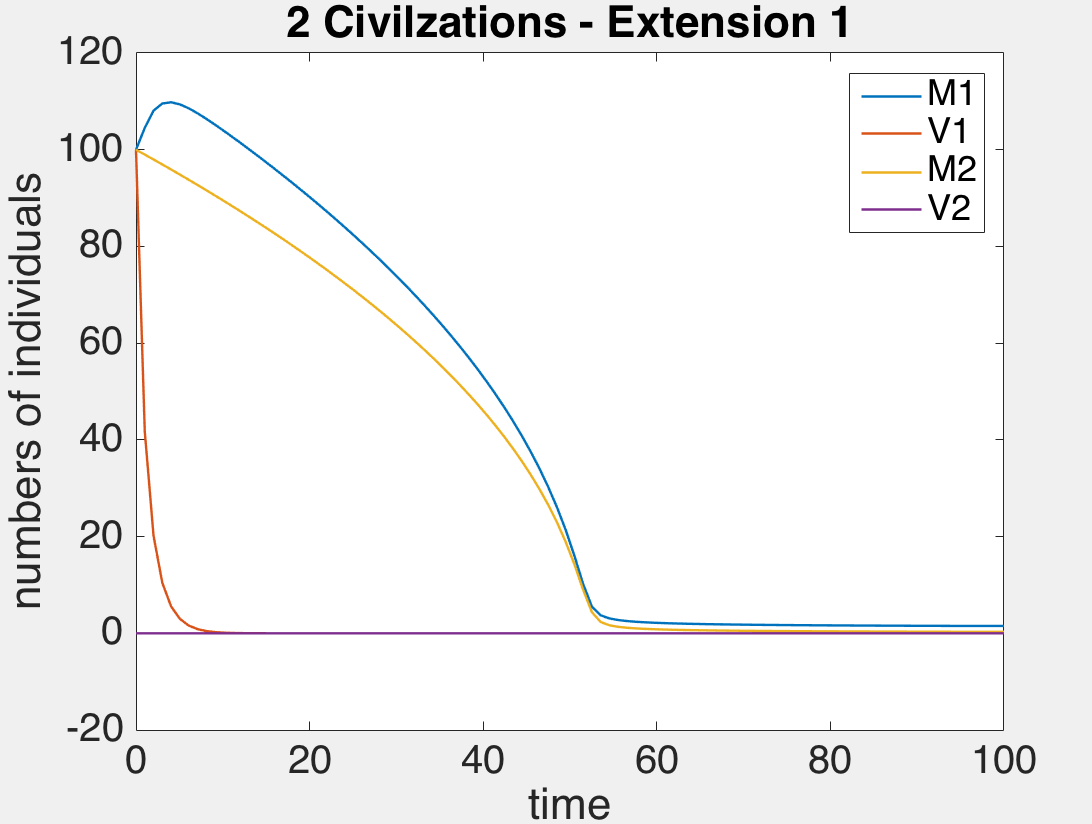
\includegraphics[width=200pt]{examplesim1}
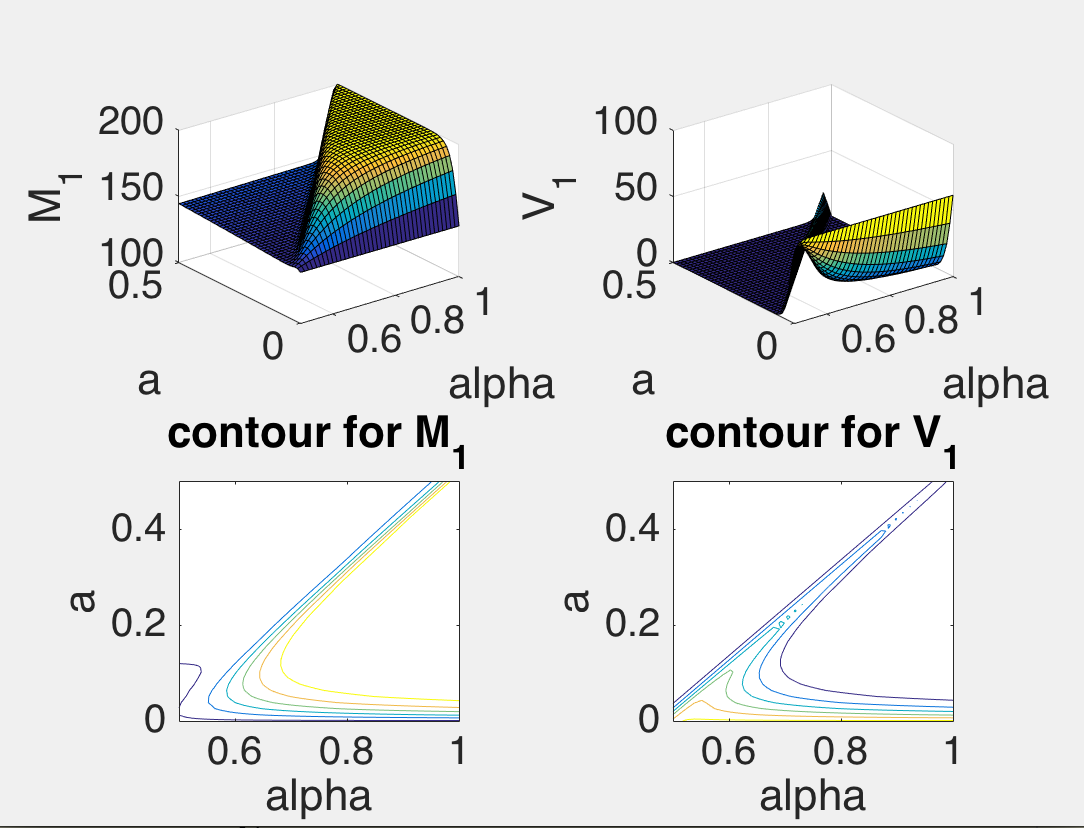
\includegraphics[width=200pt]{examplecontour1}

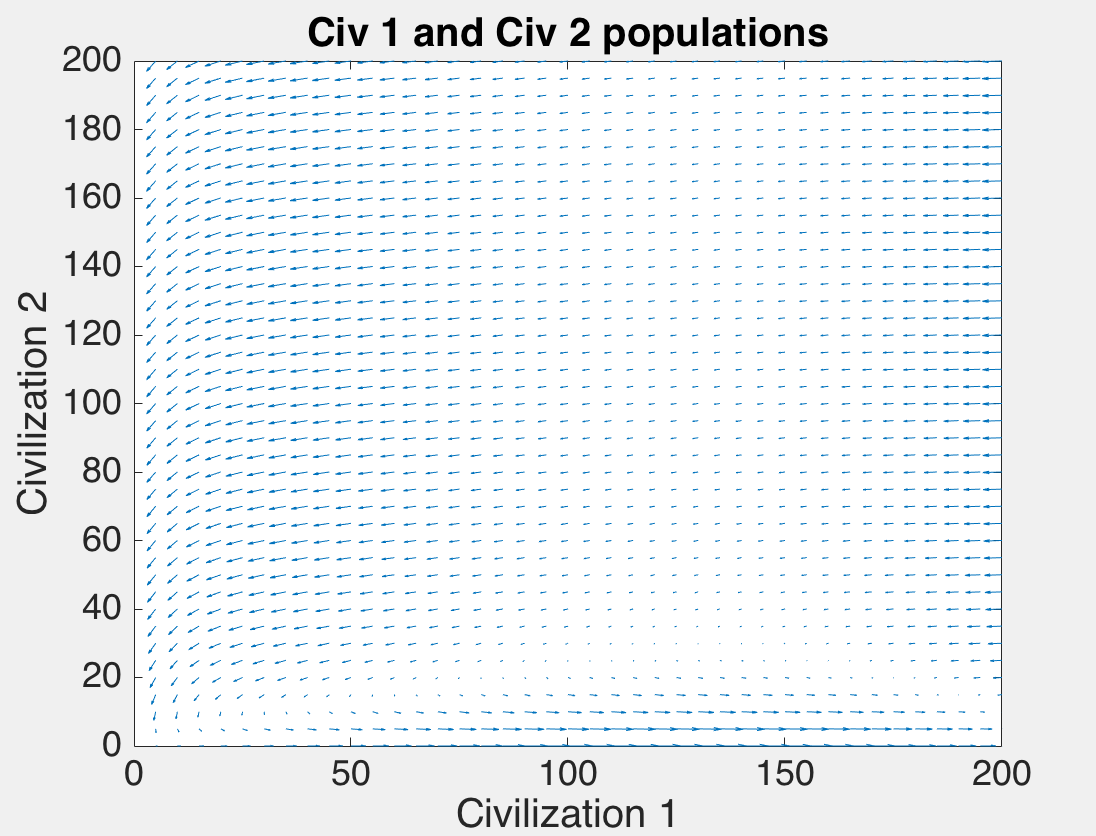
\includegraphics[width=200pt]{phase2}

\section{Discussion}
\paragraph{}

\section{Conclusion} 
\paragraph{}

\section{Attribution of Efforts} 
\paragraph{}

\section{References} 
\paragraph{}

\section{Code Appendix} 
\paragraph{}

\end{document}